\chapter{Organización de la información}

\section{Introducción}
Para abordar los problemas de coherencia propuestos en la Sección~\ref{sec:problema_coherencia-texto}, es necesario crear una estructura jerárquica para guiar el desarrollo del texto. Esta estructura está compuesta por las entidades presentes en la ontología, de manera que las entidades que consideramos más relevantes se encuentren en el primer nivel de jerarquía, y a medida que se descienda por los niveles la importancia de las entidades disminuya. Nos referiremos a esta estructura como Árbol de Entidades.

\section{Diseño}
Para organizar la información, se crearon cuatro módulos que transforman la ontología de entrada en un árbol con toda la información contenida en la ontología. A continuación se describe cada módulo:
\begin{itemize}
    \item Traductor: recibe la entrada y la traduce a una representación interna de la ontología.
    \item Clasificador de Entidades: clasifica y extrae las entidades más relevantes, utilizando como criterio las medidas de centralidad.
    \item Generador de Nuevo Grupo de Entidades: recibe una Entidad y recorre sus relaciones para crear un nuevo grupo de entidades relacionados semánticamente.
    \item Generador del Árbol de Entidades: se encarga de crear los niveles del Árbol de Entidades. 
\end{itemize}
%Para finalizar, un último módulo agrega en una nueva rama del árbol a aquellas entidades que no han sido utilizadas en ninguna otra rama.

En la Figura~\ref{fig:modulos_organizador_inf} se muestra la transformación de la ontología OWL a través de los módulos. Los pasos 4 y 5 son iterativos, el proceso finaliza cuando no queden más Entidades que explorar, lo cual es definido por el Generador del Árbol de Entidades.

\begin{figure}
    \centering
    \includegraphics%[width=12cm, height=6cm]
    [scale=1]{img/organizacion_informacion/modulos_organizador_de_informacion.pdf}
    \caption{Módulos que componen el Organizador de Información}
    \label{fig:modulos_organizador_inf}
\end{figure}


\subsection{Traductor de la entrada}
El módulo Traductor crea una representación interna de la ontología cargando toda la información en una estructura que facilita el acceso y recorrido de los datos. Como algunos datos son accedidos a través de un razonador o importados de otras ontologías, se optó por cargar toda esta información una única vez para reducir el tiempo de espera cuando se requieren estos datos.

\subsection{Clasificación de las entidades más relevantes}
Una vez creada la representación de la ontología, el segundo módulo debe clasificar las entidades y extraer las más relevantes para crear el primer nivel del Árbol de Entidades. A continuación se explicará cómo son extraídas estas entidades.

\subsubsection{Criterio de clasificación}
El criterio principal para establecer una clasificación sobre las clases de una ontología, y que tal clasificación sirva para seleccionar las clases más relevantes, se basa en cuánta información posee una clase respecto al resto de las clases en la ontología. Consideramos que una clase tiene más información que otra si está presente en más cantidad de dominios de \emph{ObjectProperties}. Esto permite reconocer las clases que tengan mayor cantidad de conexiones con otras clases, y que a su vez sean el núcleo de la relación. 

Para obtener la cantidad de información de cada clase, utilizaremos el grafo subyacente a la ontología y calcularemos el \emph{outdegree} de cada nodo que represente una clase. Para el cálculo se tendrá en cuenta únicamente la relación \emph{rdf:domain}.

Teniendo en cuenta a las clases mejor clasificadas, se puede centrar lo que se dice en el texto alrededor de estas clases.

Algunas ventajas de este enfoque son:
\begin{itemize}
    \item Sencillez de implementación. Únicamente se debe recorrer el grafo calculando el valor de cada nodo. El recorrido del grafo tiene a lo sumo una complejidad polinomial.
    \item No se requiere agregar información extra al dominio.
    \item No es necesario utilizar sobre la ontología un razonador que requiera una complejidad computacional que sea intratable. La única observación es que hay que inferir el dominio y rango de las \emph{ObjectProperties}. Sin embargo, la inferencia de dominio y rango se realiza teniendo en cuenta la jerarquía de \emph{ObjectProperties}, sin necesidad de inferir clases equivalentes o disjuntas.
\end{itemize}

La eficacia de este enfoque depende fuertemente de que las \emph{ObjectProperties} más importantes tengan el dominio explícito.


\subsubsection{Seleccionando las principales clases}
\label{sec:select_class}
Una vez calculado el valor de cada clase, se pueden seleccionar las clases que superen cierto umbral para agregarlas al primer nivel de la estructura jerárquica que guiará el desarrollo del texto. En este trabajo, se recorren todas las clases y se seleccionan las que superen el valor promedio entre cantidad de propiedades y cantidad de clases.

Si ninguna supera el valor promedio, se selecciona la o las clases con el valor más alto.

Cuando se seleccionan las clases que van a representar los temas principales, puede ocurrir que se elijan clases de una misma rama en la jerarquía de clases. Esto hace que se pierda algo de semántica, pues se incluyen clases en el mismo nivel, siendo que algunas son más específicas y pueden ser alcanzadas desde sus ancestros. Para evitar este problema, se optó por eliminar las subclases que sean seleccionadas en un principio, y que tengan a una clase ancestro dentro de los temas principales. Por ejemplo, continuando con la ontología de las pizzas, si las principales clases seleccionadas son \emph{comida} y \emph{pizza}, la clase \emph{pizza} sería eliminada del conjunto, pues es subclase de \emph{comida}. 

\subsection{Agrupando la información de las Entidades}
\label{sec:agrupando_info}
El tercer módulo crea nuevos grupos de entidades para agregar como un nuevo nivel al Árbol. Los elementos de cada grupo serán insertados como hijos de la Entidad correspondiente.

Dada una Entidad \emph{E}, debe recorrerse las relaciones de \emph{E} en la ontología, para seleccionar Entidades que serán agregadas al nuevo grupo.
El contenido de cada grupo depende del tipo de \emph{E}.
\begin{itemize}
    \item Si \emph{E} es una Clase, el nuevo grupo estará constituido por Propiedades, Individuos y Subclases. 
    \item Si \emph{E} es una Propiedad, el nuevo grupo estará constituido por Subpropiedades cuyo dominio contenga a \emph{E}, o por las clases del Rango de \emph{E} si no posee Subpropiedades.
    \item Si \emph{E} es un Individuo, no se creará ningún grupo nuevo.
\end{itemize}

Cuando existen más de una Propiedad en un grupo, se busca reemplazarlas por propiedades en común de más alto nivel en la jerarquía de propiedades. Por ejemplo, en la ontología de las pizzas, para la clase \emph{pizza} existen dos propiedades: \emph{tieneCobertura} y \emph{tieneBase}. Como estas dos propiedades tienen a su vez una \emph{superproperty} en común llamada \emph{tieneIngrediente}, se reemplaza a las dos \emph{subproperties} por su ancestro \emph{tieneIngrediente}.

En la Figura~\ref{fig:diagrama_secuencia_contentGrouping} se muestra un pseudocódigo del algoritmo usado para agrupar la información de las clases.
 
 
\begin{figure}
    \centering
    \includegraphics%[width=8cm, height=7cm]
    [scale=0.8]{img/organizacion_informacion/secuencia_contentGrouping}
    \caption{Diagrama de secuencia para agrupar la información de las clases}
    \label{fig:diagrama_secuencia_contentGrouping}
\end{figure}

\subsection{Generador Árbol de Entidades}
El cuarto módulo se encarga de crear la estructura del Árbol, sincronizando la interacción entre los demás módulos. Su objetivo es formar la jerarquía comenzando desde las Entidades más Relevantes, y agregando nuevos niveles con ayuda del Generador de Nuevos Grupos. Cuando no quedan más relaciones que recorrer en las Entidades del último nivel, revisa que todas las clases haya sido usadas al menos una vez. Si hay clases que no fueron utilizadas, invoca un algoritmo para agregar estas clases en una rama especial. Es el caso, por ejemplo, de las clases \emph{Comida} y \emph{Helado} en la ontología \emph{pizza}.

Como ejemplo, el primer y segundo nivel de la ontología de las pizzas quedaría como en la Figura~\ref{fig:macro_planning_pizza}; y el tercer nivel se muestra en la Figura~\ref{fig:macro_planning_pizza_n2}.

\begin{figure}
\centering
\begin{minipage}[c]{0.7\textwidth}
%no borrar el % de dirtree porque es necesario.
{\footnotesize 
\dirtree{%
.0 .
.1 pizza.
.2 tieneIngrediente.
.2 pizzaConCarne.
.2 pizzaConNombre.
.2 $\ldots$ las restantes subclases de pizza.
.1 comida.
.2 helado.
}}
\caption{Primer y segundo nivel del Árbol de Entidades de la ontología \emph{pizza}.}
\label{fig:macro_planning_pizza}
\end{minipage}
\end{figure}

\begin{figure}
\centering
\begin{minipage}[c]{0.7\textwidth}
%no borrar el % de dirtree porque es necesario.
{\footnotesize 
\dirtree{%
.0 .
.1 pizza.
.2 tieneIngrediente.
.3 tieneBase.
.3 tieneCobertura.
.2 pizzaConCarne.
.2 pizzaConNombre.
.3 Margherita.
.3 Napoletana.
.3 $...$ las restantes subclases de pizzaConNombre.
.2 $...$ las restantes subclases de pizza, con sus respectivas subclases.
.1 comida.
.2 helado.
}}
\caption{Tercer nivel del Árbol de Entidades de la ontología \emph{pizza}.}
\label{fig:macro_planning_pizza_n2}
\end{minipage}
\end{figure}


Se puede ver que las subproperties \emph{tieneBase} y \emph{tieneCobertura} tienen en su dominio a \emph{pizza}, la clase más cercana recorriendo sus ancestros. Si existiera por ejemplo, \emph{tieneCondimento} como una tercer subproperty de \emph{tieneIngrediente}, cuyo dominio no tuviera \emph{pizza}, entonces no sería listada dentro del grupo \emph{tieneIngredientes} en la rama de \emph{pizza}. Sin embargo, deben explorarse las subproperties de \emph{tieneCondimento}, por el caso de que tenga alguna subproperty que tuviera como dominio a \emph{pizza}. Por ejemplo, supongamos que \emph{tieneCondimento} tiene como subproperty a \emph{tieneOrégano} con diminio \emph{pizza}, en ese caso se habilita a \emph{tieneCondimento} para ser insertado en el grupo junto a  \emph{tieneCobertura} y \emph{tieneBase}. 

\subsection{Diagrama de clases}
En la Figura~\ref{fig:diagrama_clases_organizador} se muestra el diagrama de clases correspondiente al Organizador de Información. El módulo \emph{Traductor} está representado a través de la clase \emph{OntologyManager}; el módulo Clasificador de Entidades está representado por la clase \emph{ContentClasification}; el módulo que genera el Árbol de Entidades está implementado por la clase \emph{GeneratorTreeManager}, y el módulo que crea nuevos grupos de entidades está implementado en la clase \emph{ContentGrouping}. 

Las clases \emph{OWLIntClass},  \emph{OWLClass},  \emph{OWLDataProperty},  \emph{OWLObjectProperty}, \emph{OWLIndividual},\emph{OWLRestriction} y  \emph{Ontology} son usadas para representar la estructura de la ontología. Estos objetos son creados por la clase  \emph{OntologyManager}. 

\begin{figure}
    \centering
    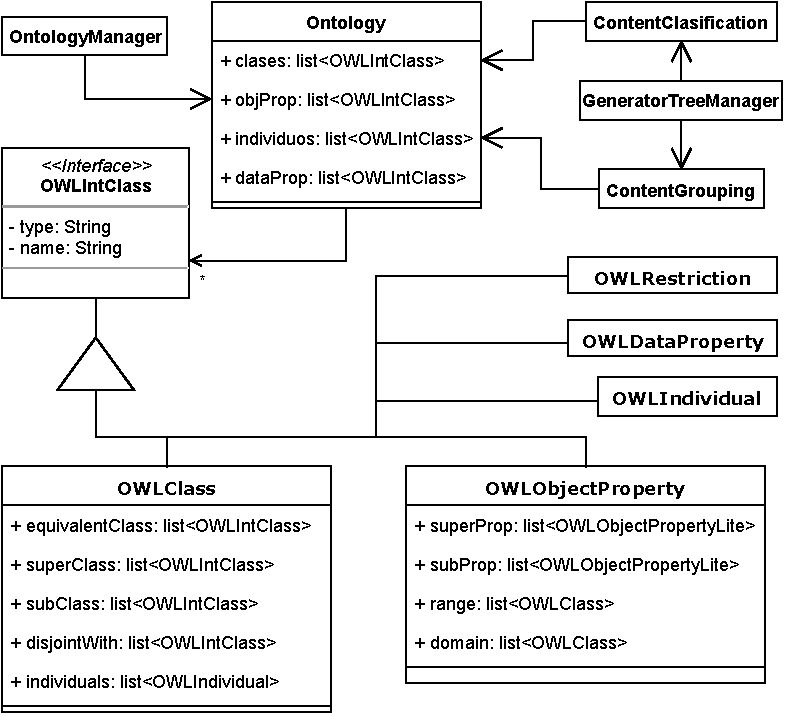
\includegraphics{img/organizacion_informacion/diagrama_clases_organizador_informacion.pdf}
    \caption{Diagrama de clases del Organizador de Información}
    \label{fig:diagrama_clases_organizador}
\end{figure}

\section{Implementación}
Para documentar la implementación se tomarán principalmente las cuatro clases asociadas a los módulos del Organizador de Información. Para simplificar la longitud de las clases documentadas, solo se mostrará el encabezado de los métodos con sus respectivas descripciones, y solo se incluirá la implementación de los métodos más importantes.

La estructura de la ontología se crea a través de la clase \emph{OntologyManager}. Esta clase hace uso de la librería  \emph{OWLAPI}\footnote{http://owlapi.sourceforge.net/} para cargar el archivo que contiene la ontología de entrada. El beneficio de esta librería es que también importa los archivos necesarios en caso de que hayan definiciones de tipo \emph{import} en la ontología. En la Figura~\ref{fig:clase_ontologymanager} se muestra un pseudocódigo del método principal de \emph{OntologyManager}.

La clase \emph{Ontology} posee la estructura creada con \emph{OntologyManager}. También posee algunos métodos útiles para el proceso de organizar la información, los cuales se muestran en la Figura~\ref{fig:clase_ontology}.

La clase \emph{ContentClasification} contiene los métodos necesarios para clasificar y extraer las entidades más relevantes. Su implementación se muestra en la Figura~\ref{fig:clase_content_clasif}.

La clase \emph{ContentGrouping} posee tres métodos para generar los grupos de nuevos tópicos del Árbol de Entidades. En la Figura~\ref{fig:clase_content_grouping} se presenta esta clase.

La clase \emph{GeneratorTreeManager} recorre recursivamente las Entidades creando las ramas del Árbol de Entidades. Se presenta un pseudocódigo en la Figura~\ref{fig:clase_generator_tree} para explicar el recorrido.

El resto de las clases solo sirven para completar la estructura en forma de grafo de la ontología, pero no agregan métodos relevantes para el Organizador de Información.

\begin{figure}
\begin{minted}[autogobble,linenos]{java}
public class OntologyManager {

    /*nameOf guarda el valor 0 o 1 para reconocer de donde tiene que
    extraer el nombre de las entidades*/
    private static int nameOf; // 0 -> iri, 1 -> label.
    /*lang setea el valor del lenguaje para buscar los nombres
    de las entidades en los labels correctos*/
    private static String lang; // "en" -> ingles, "es" -> español.

  public static Ontology createOntology
            (OWLOntology ontology, int nameOfClass, String language) {
        nameOf = nameOfClass;
        lang = language;
        Ontology onto = new Ontology();
        
        //Obtiene el título de la ontología desde la etiqueta title.
        String title = getTitleOntology();
        onto.setTitle(title);
        
        //crear clases
        OWLClass rootClass = createClasses();

        //crear los dataProperty
        OWLDataProperty rootDataProp = createDataProperty();
        
        //crear properties
        OWLObjectProperty rootProp = createObjectProperty();
        //setea las objectProperty equivalentes, inversas y disjuntas.
        setListsToProperties();
        //setea el dominio y rango de las objectProperty
        setObjectPropertyDomainRange();
        //setea el dominio y rango de las dataProperty
        setDataPropertyDomain();
        
        //crear individuals
        createIndividuals();
        
        /*crear las clases anónimas para cada clase en onto.
        Setea listas para guardar los axiomas. Para cada clase en onto
        setea sus clases equivalentes, disjuntas y superClases.*/
        /*createAnonymousClasses debe ser llamado despues de haber
        creado las clases nombradas, las properties y los individuos.*/
        createAnonymousClasses();
        
        //agrega los componentes creados al objeto onto.
        addComponentsToOnto();
        
        //precomputeValues asocia a cada clase en onto una lista 
        //de propiedades en las que participa como dominio.
        onto.precomputeValues();
        return onto;
    }
}
\end{minted}
\caption{Definición en Java de la Clase \texttt{OntologyManager}.}
\label{fig:clase_ontologymanager}
\end{figure}


\begin{figure}
\begin{minted}[autogobble,linenos]{java}
public class Ontology {

    private String title;
    //guardan las Entidades de nivel mas alto en la jerarquía.
    private OWLClass rootClass;
    private OWLObjectProperty rootObjectProperty;
    private OWLDataProperty rootDataProp;

    //los siguientes hashmaps asocian IRIs a sus respectivas Entidades.
    private HashMap<IRI, OWLClass> classes;
    private HashMap<IRI, OWLObjectProperty> properties;
    private HashMap<IRI, OWLObjectProperty> anonProperties;
    private HashMap<IRI, OWLDataProperty> dataProperties;
    private HashMap<IRI, OWLIndividual> individuals;
    
    //Las siguientes listas guardan las Entidades presentes en la 
    //ontologia
    private LinkedList<OWLClass> listClasses;
    private LinkedList<OWLObjectProperty> listProps;
    private LinkedList<OWLObjectProperty> anonListProps;
    private LinkedList<OWLDataProperty> listDataProps;
    private LinkedList<OWLIndividual> listIndividuals;

    /*hashmaps para guardar que clases participan en el dominio
    de que propiedades*/
    HashMap<OWLClass, LinkedList<OWLObjectProperty>> classOnPropDomain;
    /*hashmaps para guardar que clases participan en el rango
    de que propiedades*/
    HashMap<OWLClass, LinkedList<OWLObjectProperty>> classOnPropRange;

    /*Retorna una lista de ObjectProperties que sean superProperties
    en comun de las properties de la lista prop.*/
    public LinkedList<OWLObjectProperty>
    getCommonSuperProperties(LinkedList<OWLObjectProperty> prop) {}

    /*Dada la clase cls, recorre las properties donde participa como dominio
    y busca las superProperties de mas alto nivel que encuentre 
    y las retorna. */
     public LinkedList<OWLObjectProperty>
     getCommonSuperPropertiesFromClass(OWLClass cls) {}

    /*Retorna el contenido necesario para crear un nuevo grupo
    de entidades a partir de la clase cls. Util para
    el modulo ContentGrouping */
    public LinkedList<OWLIntClass> 
    createTopicsGroupsFromClass(OWLClass cls) {
        LinkedList<OWLIntClass> res = new LinkedList<>();
        res.addAll(getCommonSuperPropertiesFromClass(cls));
        res.addAll(cls.getSubClass());
        res.addAll(cls.getIndividuals());
        return res;
    }
}
\end{minted}
\caption{Definición en Java de la Clase \texttt{Ontology}.}
\label{fig:clase_ontology}
\end{figure}


\begin{figure}
\begin{minted}[autogobble,linenos]{java}

public class ContentClasification {

    /* Es el método principal que retorna las entidades
    más relevantes para agregar en el primer nivel de
    la jerarquía del Árbol de Entidades. */
    public static HashMap<OWLIntClass, LinkedList<OWLObjectProperty>>
    getMainContent(Ontology ontology) {
        
        cls2Cant = getClassesToCantProperties(ontology);
        mainClasses = getMainClasses(cls2Cant);

        /*insertar en un nuevo hashmap cls2SuperProp las clases de mainClasses
        asociadas a las superProperties en común que haya entre las properties 
        donde participa como dominio*/
        for (OWLClass mainClass : mainClasses) {
            cls2SuperProp.put(mainClass,
            ontology.getCommonSuperPropertiesFromClass(mainClass));
        }
        
        /*Si existe una Clase c y alguna SuperClase de c, 
        entonces c se elimina por ser mas específica*/
        cls2SuperProp = removeSubClass(cls2SuperProp);

        /*si el hashmap es vacio, entonces se agregan todas las
        clases sin objproperties*/
        if (cls2SuperProp.isEmpty()) {
            for (OWLClass cls : ontology.getClasses()) {
                cls2SuperProp.put(cls, new LinkedList<>());
            }
        }
        return cls2SuperProp;
    }
    
    /*Devuelve una Lista de HashMaps desde Clases a Integers. Cada
     Hashmap tiene una sola entrada, que va desde una Clase a la
     cantidad de properties en las que participa como dominio.*/
    private static LinkedList<HashMap<OWLClass, Integer>>
    getClassesToCantProperties(Ontology ontology) {}
    
    /*Devuelve una lista de Clases. Las Clases retornadas son las
     que participan en mas cantidad de properties, y que superan 
     el promedio calculado como la suma de todas las properties
     dividido entre la cantidad de clases.*/
    private static LinkedList<OWLClass>
    getMainClasses(LinkedList<HashMap<OWLClass, Integer>> cls) {}
}

\end{minted}
\caption{Definición en Java de la Clase \texttt{ContentClasification}.}
\label{fig:clase_content_clasif}
\end{figure}


\begin{figure}
\begin{minted}[autogobble,linenos]{java}
public class ContentGrouping {

    /*A partir de la clase cls y la rama branch a la que pertenece,
    se genera un nuevo grupo de Entidades, y se verifica que cada
    Entidad aún no pertenezca a la rama*/
    public static LinkedList<OWLIntClass>
    generateNewTopics(Ontology ontology, OWLClass cls, 
                LinkedList<OWLIntClass> branch) {
        LinkedList<OWLIntClass> tops = ontology.createTopicsGroupsFromClass(cls);
        for (OWLIntClass r : tops) {
            if (!r.getType().equals("property")) {
                    if (!branch.contains(r)) {
                        res.add(r);
                    }
            }
        }
        for (OWLIntClass r : tops) {
            if (r.getType().equals("property")) {
                checkProperties((OWLObjectProperty) r, res, branch);
            }
        }
        return res;
    }

    /*A partir de una property prop y la clase dom que pertenece
    a su dominio, busca crear un nuevo grupo de Entidades.
    Primero busca subProperties de prop. Si no tiene subProperties, 
    entonces intenta agregar el Rango de prop.*/
    public static LinkedList<OWLIntClass> 
    generateNewTopics(Ontology ontology, OWLObjectProperty prop,
                    OWLClass dom) {
        
        /*obtiene las subProperties de prop*/
        LinkedList<OWLIntClass> newTopics = prop.getSubPropWithDomain(dom);
        
        if (newTopics.isEmpty()) {
            newTopics = prop.getRange();
        }
        return newTopics;
    }
    
    /*A partir de prop busca agregar a ella o una superProperty
    de ella en res. Agrega a prop si tiene una superProperty en branch.
    Si no puede agregar a prop busca agregar un ancestro de prop que 
    tenga una superProperty en branch.*/
    private static boolean checkProperties(OWLObjectProperty prop,
    LinkedList<OWLIntClass> res, LinkedList<OWLIntClass> branch) {}
}
\end{minted}
\caption{Definición en Java de la Clase \texttt{ContentGrouping}.}
\label{fig:clase_content_grouping}
\end{figure}


\begin{figure}
\begin{minted}[autogobble,linenos]{java}
public class GeneratorTreeManager {

    public static LinkedList<OWLIntClass> getText(Ontology onto) {

        HashMap<OWLIntClass, LinkedList<OWLObjectProperty>> mainClass =
        ContentClasification.getMainContent(onto);
        
        /*agregar las clases de mainClass al primer nivel del árbol. 
        mainEntities representa el primer nivel del árbol 
        (las entidades mas relevantes)*/
        mainEntities.add(mainClass);
        
        /*para cada clase de mainClass crear una nueva rama y agregar 
        sus Nuevos grupos de Entidades*/
        for (Map.Entry<OWLIntClass, LinkedList<OWLObjectProperty>> entrySet : 
                mainClass.entrySet()) {
            /*navigation mantiene las clases del primer nivel y
            las Entidades de la rama que se está creando*/
            navigation.add(mainClass);
            OWLClass mClass = entrySet.getKey();
            LinkedList<OWLIntClass> newEntities =
            ContentGrouping.generateNewTopics(onto, mClass, null);
            addBranchFromEntity(newBranch, mClass, newEntities, navigation,
            onto);
            mainEntities.addNewBranchToEntity(mClass, newBranch);
            navigation.clear();
            
        }
        /*agregar informacion marginada*/
        mainEntities.addNewBranch(addAbsentClass(onto));
        return mainEntities;
    }
    
    /*Recorre las newEntities creando sus respectivos niveles de jerarquía 
    en el Árbol de Entidades.*/
    private static void addBranchFromEntity(newBranch, OWLClass actualClass,
    newEntities, navigation, onto) {
        for (OWLIntClass enti : newEntities) {
            if (!navigation.contains(enti)) {
                navigation.addLast(enti);
                if (enti.getType().equals("class")) {
                    sub2 = ContentGrouping.generateNewTopics(onto, enti, navigation);
                    addBranchFromEntity(newSubBranch, enti, sub2, navigation, onto);
                }else if (enti.getType().equals("property")) {
                    sub2 = ContentGrouping.generateNewTopics(onto, enti, actualClass);
                    addBranchFromEntity(newSubBranch, actualClass, sub2, navigation, onto);
                }
                navigation.removeLast();
                newBranch.addNewBranchToEntity(enti, newSubBranch);
            }
        }
    }
}

\end{minted}
\caption{Definición en Java de la Clase \texttt{GeneratorTreeManager}.}
\label{fig:clase_generator_tree}
\end{figure}


\section{Casos de estudio}
En esta sección se presentan dos casos de estudio que muestran el comportamiento de la aplicación ante dos entradas diferentes, abarcando distintos aspectos de la solución propuesta. En el primer caso será usada la ontología de las pizzas, y en el segundo se hará uso de la ontología \emph{Wine}\footnote{https://www.w3.org/TR/owl-guide/wine.rdf}.

Al momento de realizar este trabajo no se reconoce ninguna aplicación que aborde el problema de organización de la información en una ontología, por lo que se expondrán tres casos de estudio sin la posibilidad de compararlos con otros resultados.

\subsection{Organización de Ontología Pizza}
Según la descripción de la ontología, este dominio representa las pizzas y sus coberturas, por lo que esperamos que las entidades que representen a las pizzas, a las coberturas y la información complementaria tiendan a agruparse en los niveles más altos de la jerarquía, mientras que en los niveles más bajos esperamos encontrar las clases más específicas y que tienen menor impacto sobre el entendimiento del dominio.

En la Figura~\ref{fig:caso_estudio_pizza} se puede ver el resultado de aplicar el algoritmo teniendo como entrada la ontología pizza. 

Los nombres de las entidades fueron traducidos al español, para poder generar las sentencias en lenguaje español en el siguiente capítulo, pero el idioma no afecta los resultados del algoritmo propuesto.

\begin{figure}
\begin{multicols}{2}
\begin{figure}[H]
\dirtree{%
.1 Pizza.
.2 Pizza con nombre.
.3 Margherita.
.3 Frutti di mare.
.3 Giardiniera.
.3 ....
.3 Napoletana.
.2 Pizza con carne.
.2 Pizza picante.
.2 ....
.2 Pizza vegetariana.
.2 Ingredientes.
.3 Coberturas.
.4 Cobertura de pizza.
.5 Cobertura de verduras.
.6 Cobertura de pimiento.
.6 ....
.6 Cobertura de langostinos.
.3 Bases.
.4 Base de pizza.
.5 Base gruesa.
.5 Base delgada y crujiente.
}
\end{figure}

\begin{figure}[H]
\dirtree{%
.1 Otras secciones.
.2 Domain concept.
.3 Comida.
.4 Helado.
.4 Ingrediente.
.3 Pais.
.4 America.
.4 England.
.4 Italy.
.4 France.
.4 Germany.
.2 Value partition.
.3 Picante.
.4 Poco picante.
.4 Algo picante.
.4 Muy picante.
}
\end{figure}
\end{multicols}
\caption{Resultado del Organizador de Información con la ontología \emph{Pizza}.}
\label{fig:caso_estudio_pizza}
\end{figure}

La ontología pizza cuenta con 100 clases y 8 propiedades. De las 8 propiedades, 5 fueron usadas  para clasificar las 100 clases (de las 8, 3 eran inversas a otras 3 por lo que no agregaban información nueva). El promedio de información obtenido fue 1.25, siendo la clase Pizza la única en superar este valor, lo que concuerda con el resultado esperado.

Como se puede observar en la Figura~\ref{fig:caso_estudio_pizza}, en la primer columna se encuentran los tópicos principales reconocidos por el algoritmo, y en la segunda columna se encuentra una rama especial, para aquellas clases que no habían sido utilizadas en el resto del árbol.

En la jerarquía de los tópicos principales, se puede ver como toda la información se agrupa como hijas de la entidad Pizza, describiendo los tipos de pizzas y sus ingredientes. Inmediato a los ingredientes lista las coberturas, y reconoce a las bases de pizza a la misma altura que las coberturas, asignándoles la misma importancia.

En la jerarquía de \emph{otras secciones}, se aprecian las demás entidades que aportan información secundaria a la descripción del dominio, que no está directamente relacionada con el dominio de las pizzas, como son los países, los tipos de picante y otras comidas.

Respecto al resultado esperado, la organización de la información es satisfactoria, ya que se asimila a la propia descripción del dominio. 

\subsection{Organización de Ontología Wine}
Esta ontología tiene como objetivo describir un dominio de vinos y comidas\footnote{\url{https://protege.stanford.edu/publications/ontology_development/ontology101-noy-mcguinness.html}}, por lo que esperamos que las entidades que se consideren más relevantes sean aquellas afines a los vinos y comidas.

En la Figura~\ref{fig:caso_estudio_wine} se puede ver el resultado de aplicar el algoritmo.

\begin{figure}
\begin{multicols}{2}
{\small
\begin{figure}[H]
\dirtree{%
.1 Wine.
.2 Italian wine.
.3 Chianti.
.4 Chianti classico.
.2 $...$ \emph{(otras subclases de Wine)}.
.2 Wines descriptor.
.3 Sugar.
.4 Wine sugar.
.5 Dry.
.5 Off dry.
.5 Sweet.
.3 Colors.
.4 Wine color.
.5 White.
.5 Rose.
.5 Red.
.3 Flavors.
.4 Wine flavor.
.5 Moderate.
.5 Strong.
.5 Delicate.
.3 Bodies.
.4 Wine body.
.5 Medium.
.5 Full.
.5 Light.
.2 From grapes.
.3 Wine grape.
.4 Chenin blanc grape.
.4 $...$ \emph{(otras subclases de Wine grape)}.
}
\end{figure}}  

\begin{figure}[H]
\dirtree{%
.1 Otras secciones.
.1 Region.
.2 Central texas region.
.2 $...$ \emph{(otras subclases de Region)}.
.1 Vintage year.
.2 Year1998.
.1 Wine descriptor.
.2 Wine taste.
.1 Non consumable thing.
.1 Vintage.
.2 Vintage years.
.1 Fruit.
.1 Winery.
.2 Chateau de meursault.
.2 $...$ \emph{(otras subclases de Winery)}.
.1 Consumable thing.
.2 Meal.
.3 Courses.
.4 Meal course.
.5 Cheese nuts dessert course.
.5 $...$ \emph{(otras subclases de Meal course)}.
.5 Foods.
.6 Edible thing.
.7 Fowl.
.8 $...$.
.7 Dessert.
.8 $...$.
.7 Meat.
.8 $...$.
.7 Seafood.
.8 $...$.
.7 Sweet fruit.
.8 Grape.
.8 $...$.
.7 Pasta.
.8 $...$.
.7 Non sweet fruit.
.5 Drinks.
.6 Potable liquid.
.7 Juice.
.7 Wine.
.8 Wines descriptor.
.8 From fruits.
}
\end{figure}

\end{multicols}
\caption{Resultado del organizador de información con la ontología Wine.}
\label{fig:caso_estudio_wine}
\end{figure}


La ontología Wine cuenta con 138 clases y 16 propiedades. De las 16 propiedades, 12 fueron usadas para verificar qué clases superan el promedio para ser seleccionadas como las principales. El promedio fue de 2.5 y la única clase que lo superó fue Wine, lo que cumple parcialmente el resultado esperado, ya que parte del objetivo de la ontología es describir el dominio de los vinos. Respecto a la sección que describe las comidas, quedó desplazada a \emph{otras secciones}, siendo un resultado no esperado según el objetivo de la ontología. Sin embargo, analizando manualmente la ontología, se puede apreciar que el porcentaje de  información que describe a las comidas es significativamente menor en relación a la información referida a los vinos, factor por el cual resulta aceptable que no aparezcan como sección principal.

%\subsection{Organización de Ontología SNOMED-CT}

\section{Conclusiones}
Abordamos el problema de organizar la información de una ontología, tratando de maximizar la coherencia de la estructura generada. Como planteamos inicialmente, tuvimos que definir:
\begin{itemize}
    \item Las entidades que iban a representar los nodos de la estructura: donde elegimos para el primer nivel de la jerarquía a las Clases, y para los próximos niveles a Clases, Propiedades e Individuos.
    \begin{itemize}
        \item El criterio para ponderar la importancia de las Clases para crear el primer nivel: donde decidimos usar el criterio de centralidad de un nodo, teniendo en cuenta solo la relación \emph{rdfs:domain}.
    \end{itemize}
    \item El recorrido de la ontología para crear los siguientes niveles: para el cual seleccionamos las relaciones \emph{rdfs:Domain}, \emph{owl:subPropertyOf}, \emph{rdfs:Range} y \emph{rdfs:subClassOf}. El recorrido para cada Entidad visita todos sus vecinos a solo un nivel de profundidad.
\end{itemize}

Los resultados fueron satisfactorios, obteniendo estructuras que corresponden a los resultados esperados. 

Si bien el resultado de la clasificación de las entidades mas importantes depende de la cantidad de \emph{owl:ObjectProperties} y de que sus \emph{rdfs:domain} estén correctamente establecidos, en general el hecho de que son Redes Libres de Escala es un punto a favor para este enfoque.